
As was shown in previous analysis,
signal peptides tend to promote helix formation and demote coil formation near the N-terminal end of the protein (Fig. \ref{fig:twin_helix}, \ref{fig:twin_coil}).
Little effect was seen on the propensity toward sheet formation (Fig. \ref{fig:twin_sheet}).
In addition, the signal peptide seems to have a stabilizing effect on backbone dynamics near the N-terminal end (Fig. \ref{fig:twin_backbone}).
Overall, there seems to be a higher propensity toward helix formation and backbone rigidity in cytoplasmic than periplasmic proteins.
Interestingly, previous analysis showed that periplasmic proteins have a higher tendency toward coil formation from residue 20 to 70 (red,yellow and blue region), with dip near residue 33 (yellow region).
This also shows in the twin analysis (Fig. \ref{fig:twin_coil}),
were there seems to be an slight preference for coil formation in periplasmic proteins, 
except for region near residue 33 where there is clear decrease in preference.
In the previous analysis this yellow regions near residue 33 showed a clear peak in propensity toward sheet formation for periplasmic proteins.
This is not observed in the twin analysis, 
instead periplasmic proteins display an increased preference for helix formation.
At the same position, an increased preference for early folding is observed in periplasmic proteins,
as well as increased sidechain rigidity.
This suggests that the region near position 33 plays an important role in translocation toward the periplasm,
as it folds earlier with an decreased preference to form a coil.

~\begin{figure}[h!]
	~\begin{subfigure}[b]{\linewidth}
			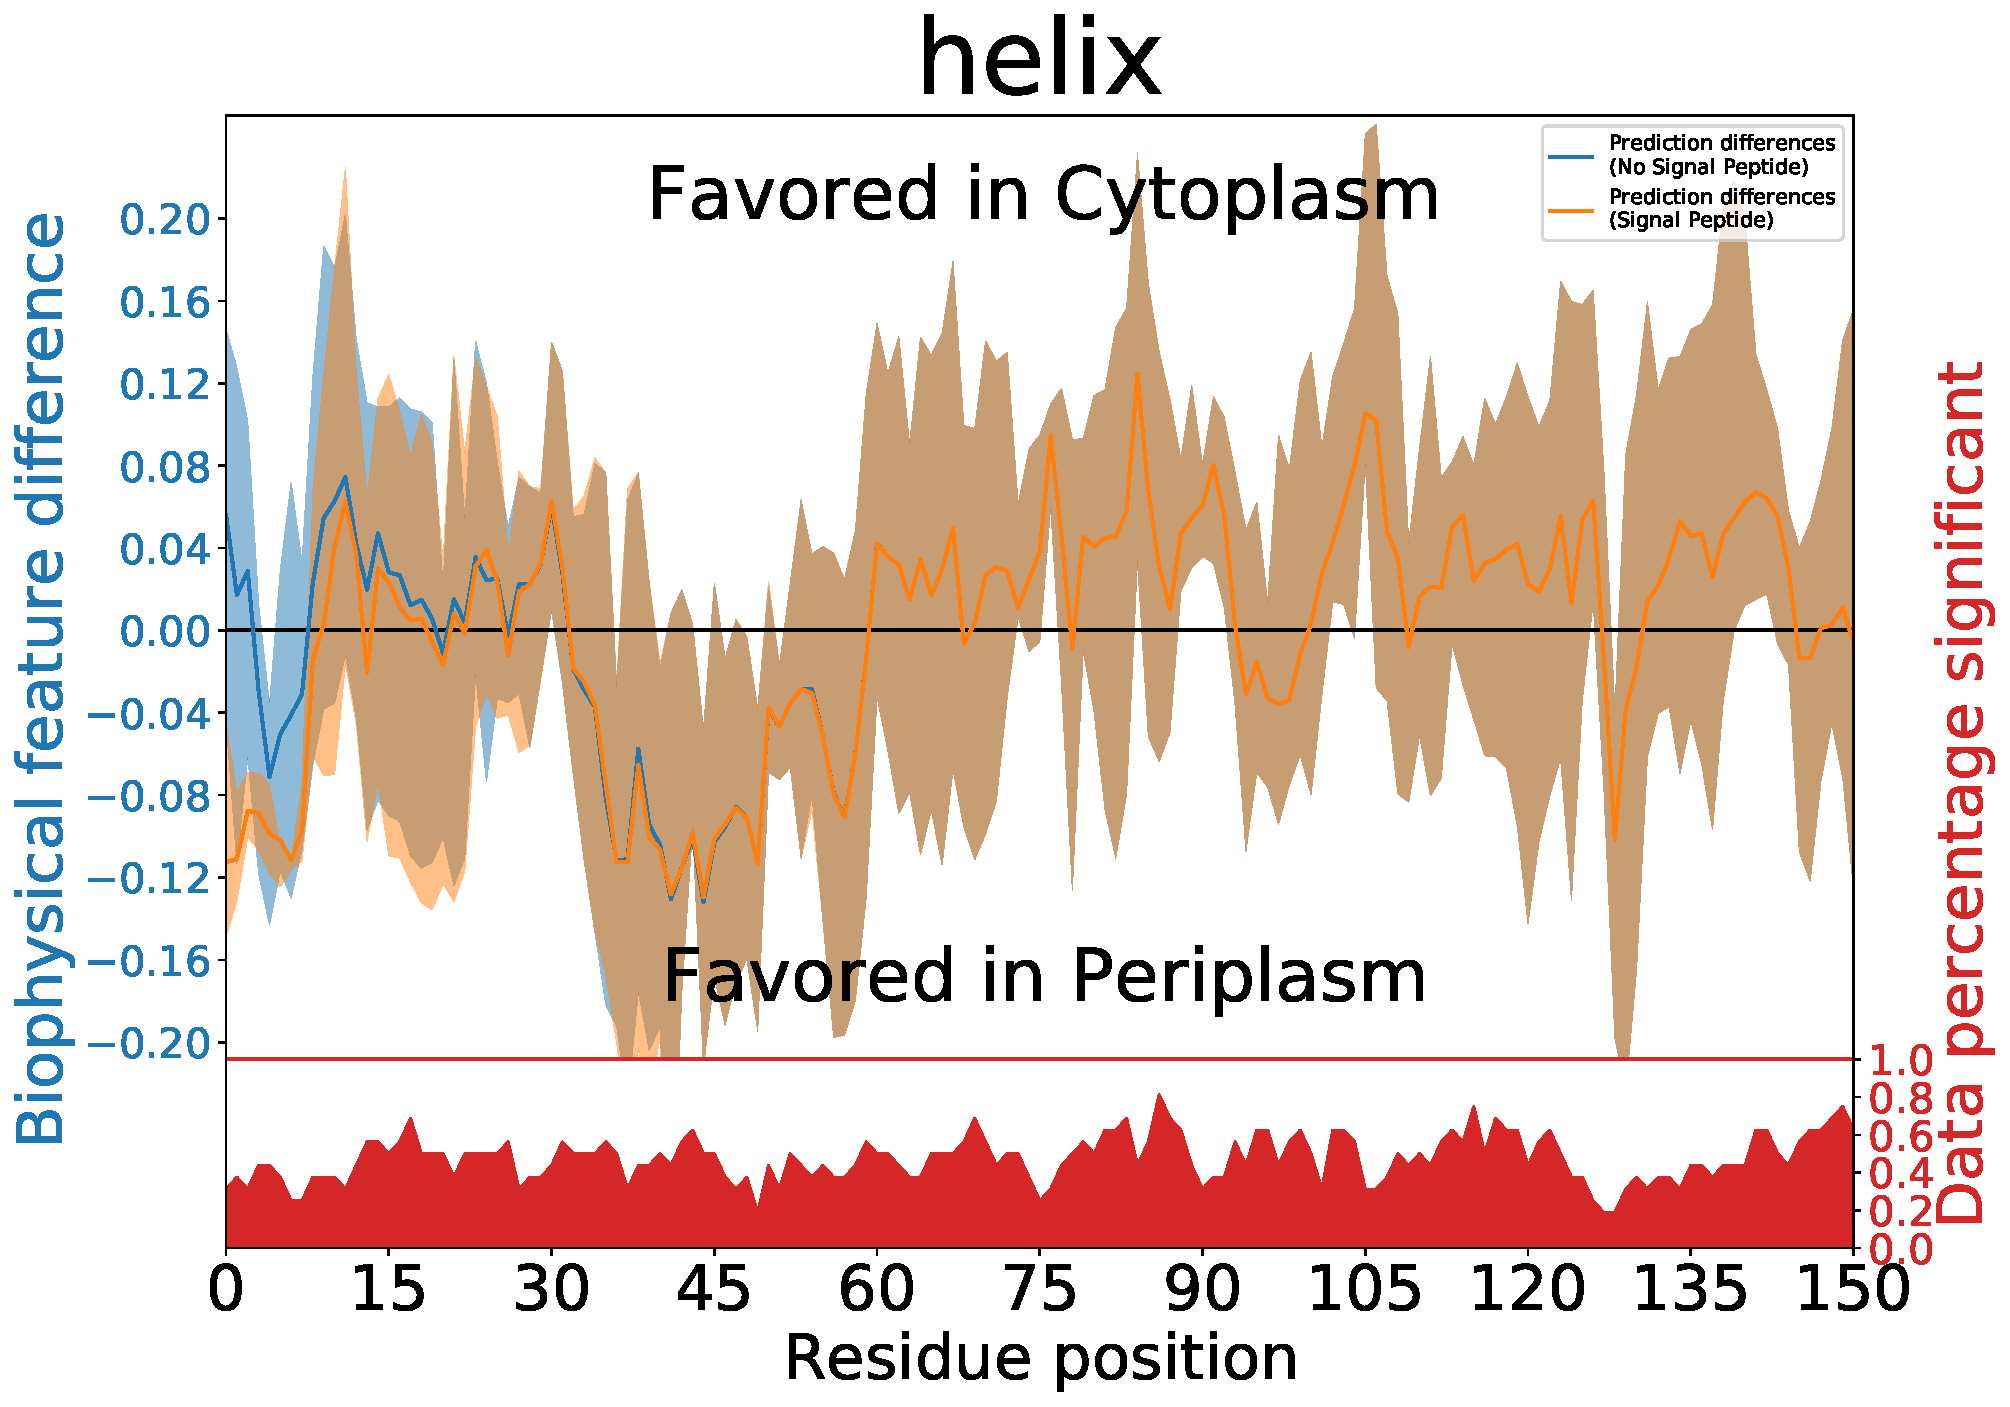
\includegraphics[width=\linewidth, height=0.43\textheight, keepaspectratio]
	{./results/twins/img/helix.pdf}
		\caption{}
		\label{fig:twin_helix}
	~\end{subfigure}
	\newline
	~\begin{subfigure}[b]{\linewidth}
			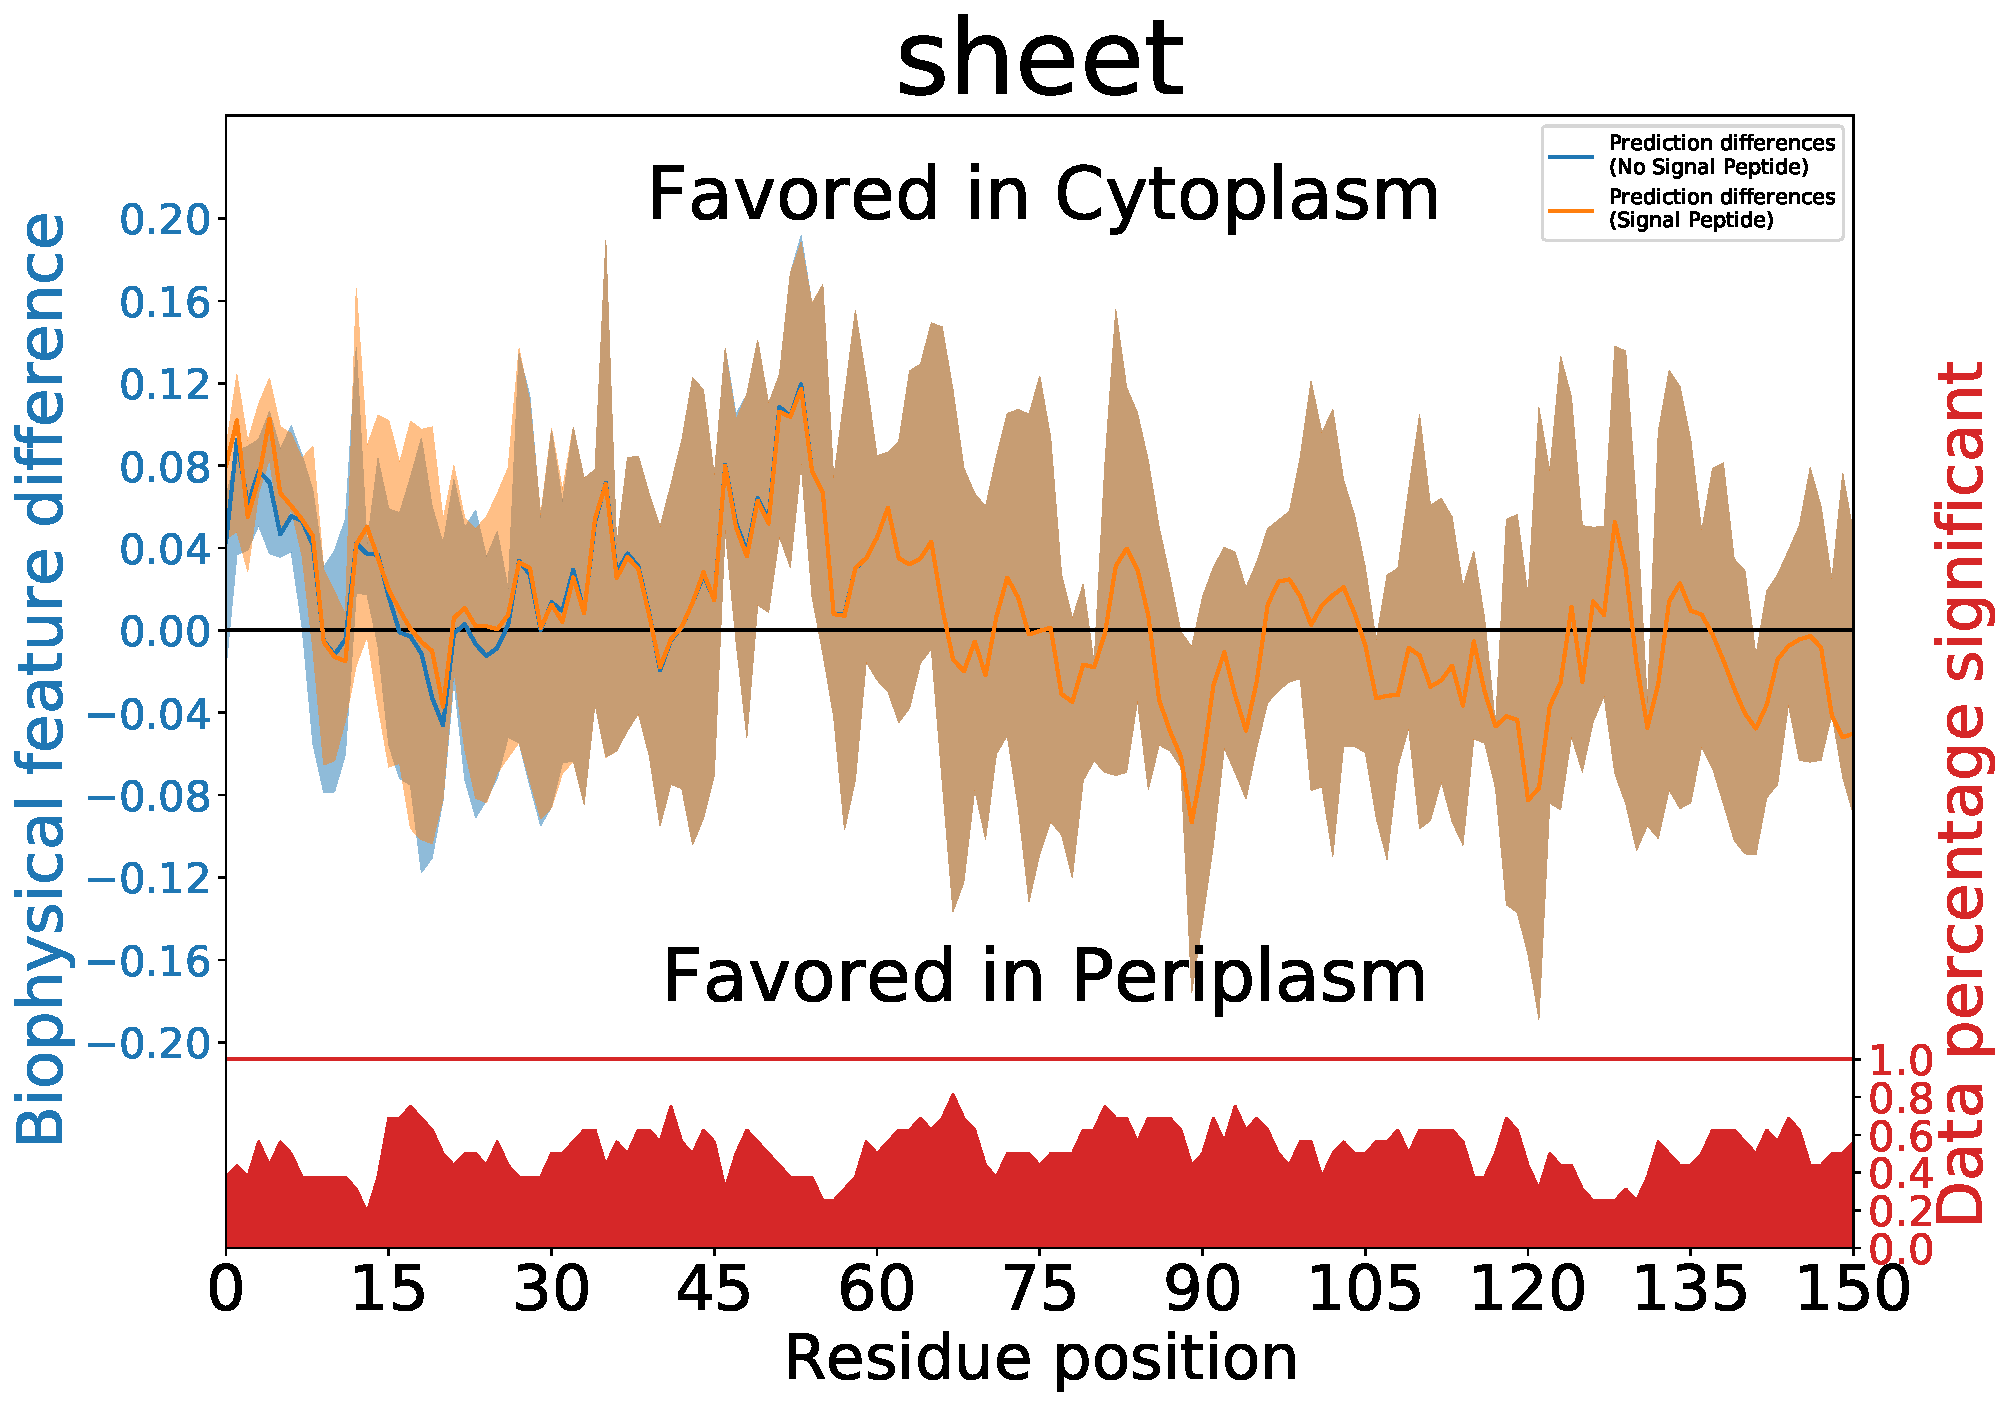
\includegraphics[width=\linewidth, height=0.43\textheight, keepaspectratio]
	{./results/twins/img/sheet.pdf}
		\caption{}
		\label{fig:twin_sheet}
	~\end{subfigure}
~\end{figure}


~\begin{figure}[h!]
	\ContinuedFloat
	~\begin{subfigure}[b]{\linewidth}
		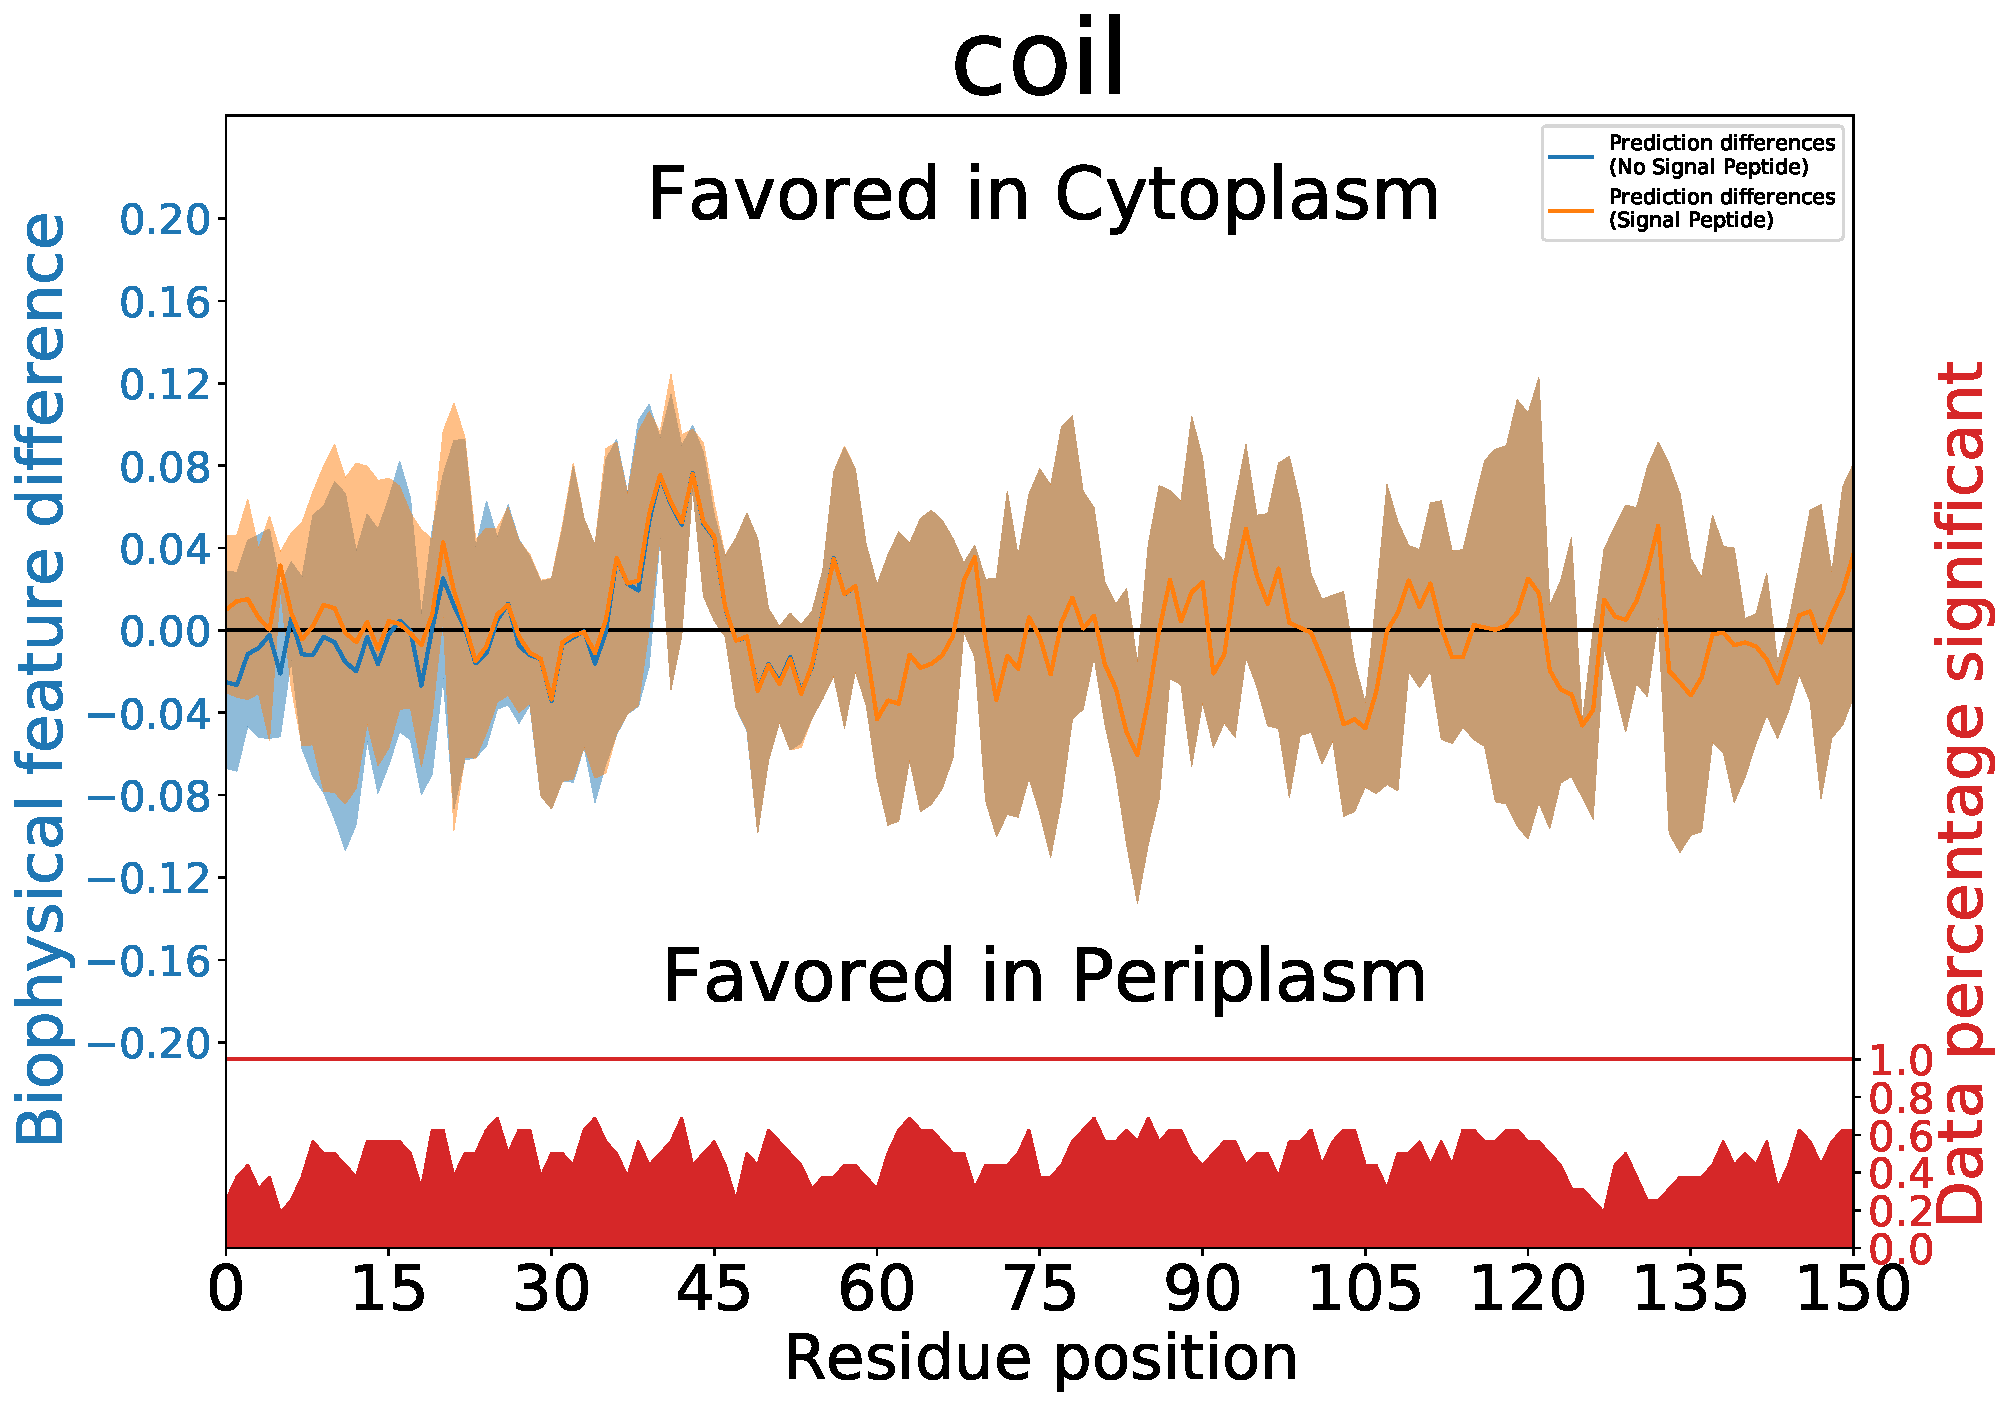
\includegraphics[width=\linewidth, height=0.43\textheight, keepaspectratio]
	{./results/twins/img/coil.pdf}
		\caption{}
		\label{fig:twin_coil}
	~\end{subfigure}
	\newline
	~\begin{subfigure}[b]{\linewidth}
			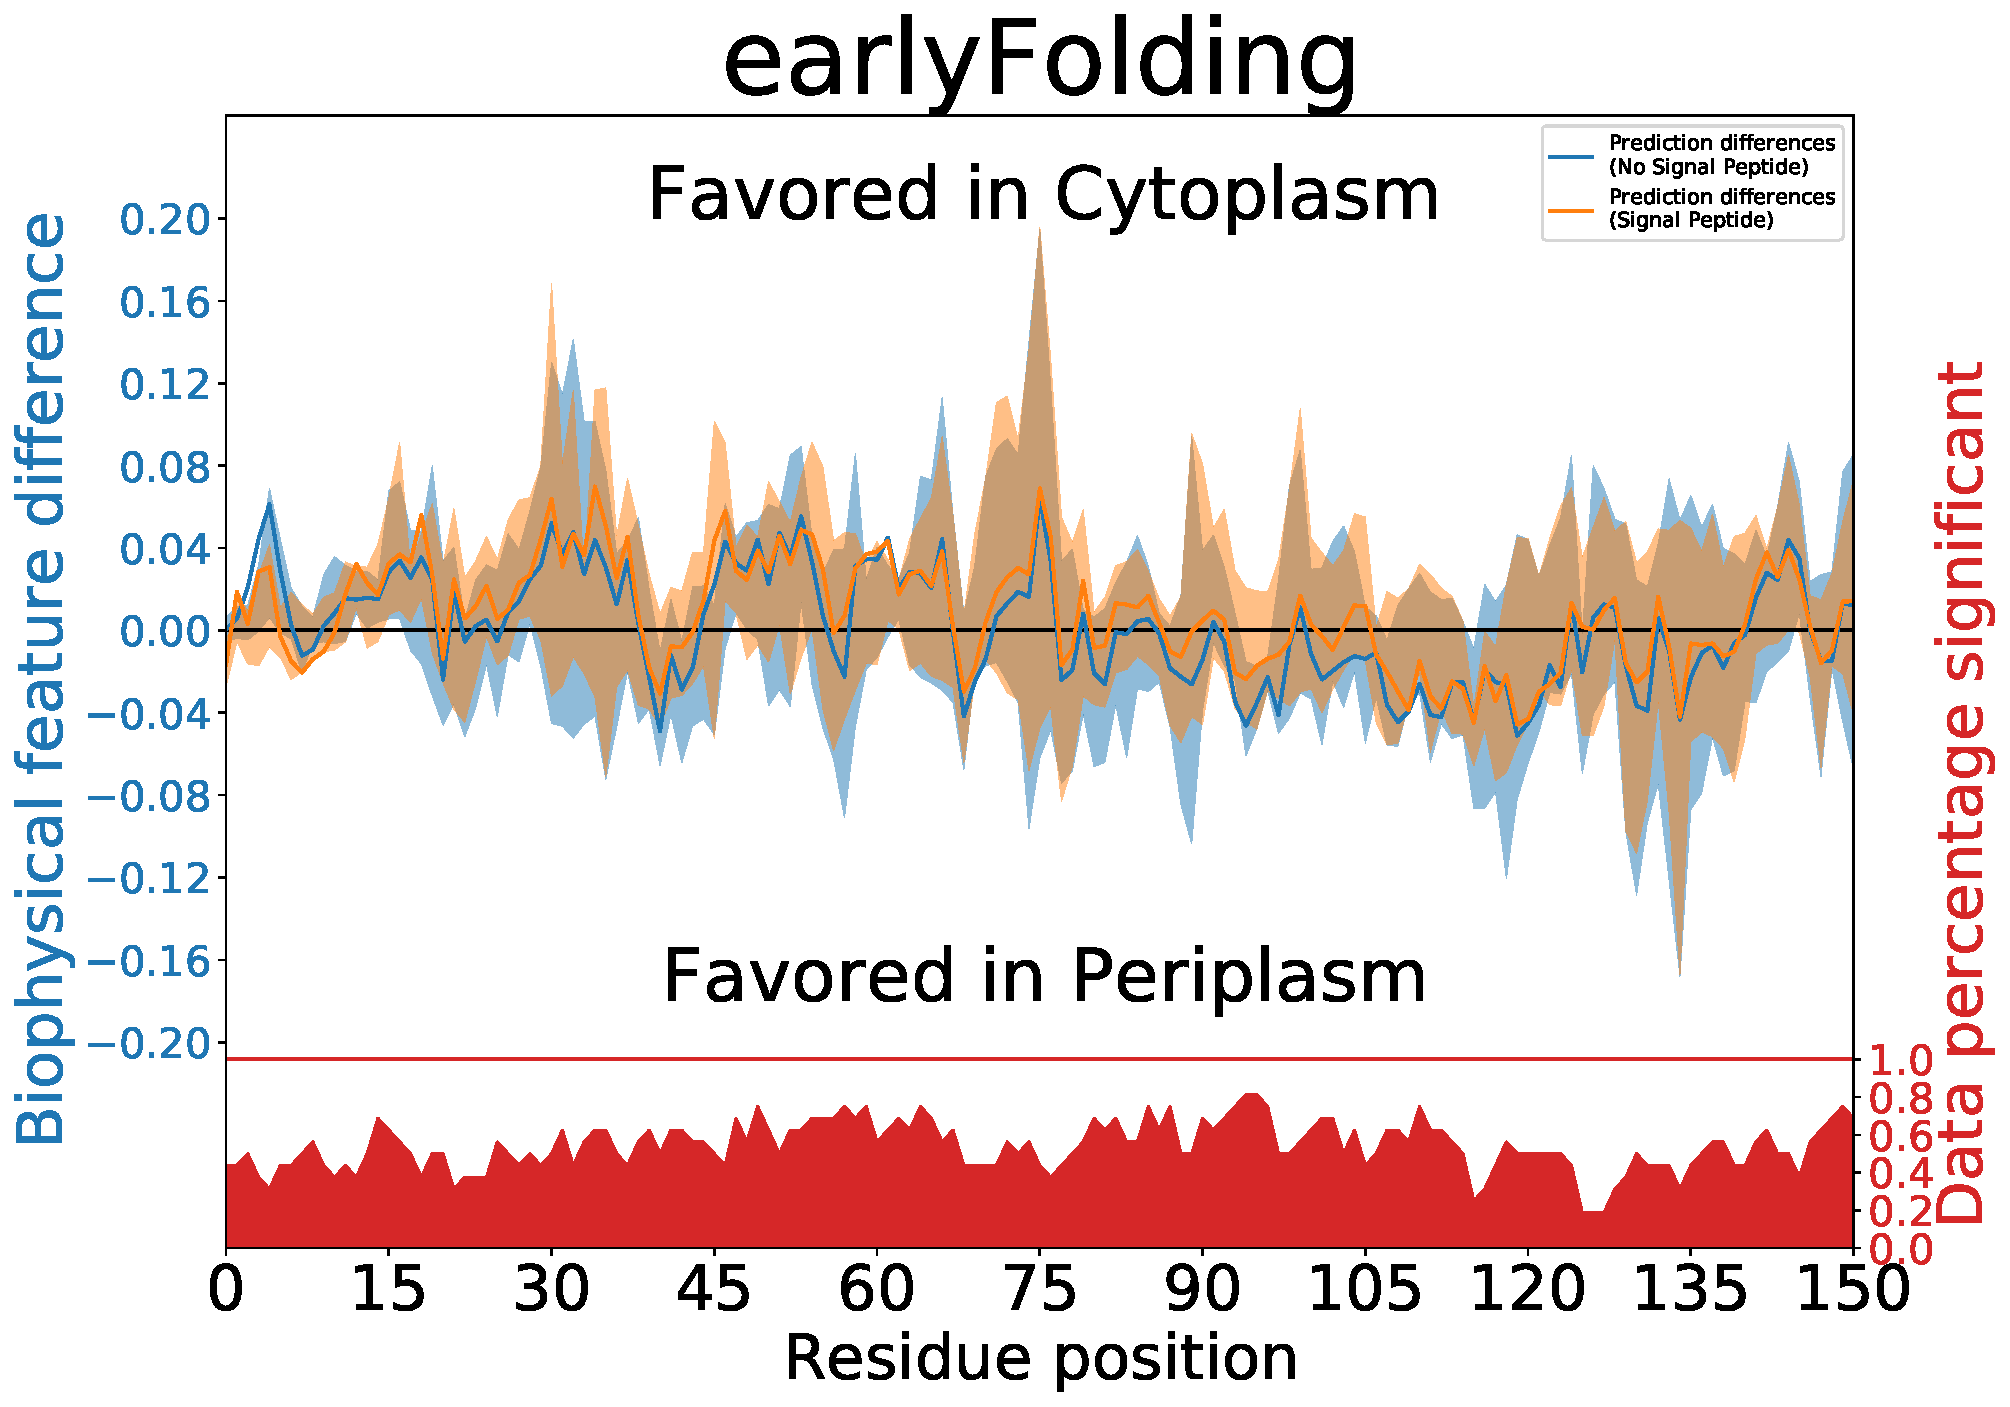
\includegraphics[width=\linewidth, height=0.43\textheight, keepaspectratio]
	{./results/twins/img/earlyFolding.pdf}
		\caption{}
		\label{fig:twin_earlyfolding}
	~\end{subfigure}
~\end{figure}


~\begin{figure}[h!]
	\ContinuedFloat
	~\begin{subfigure}[b]{\linewidth}
			\centering
			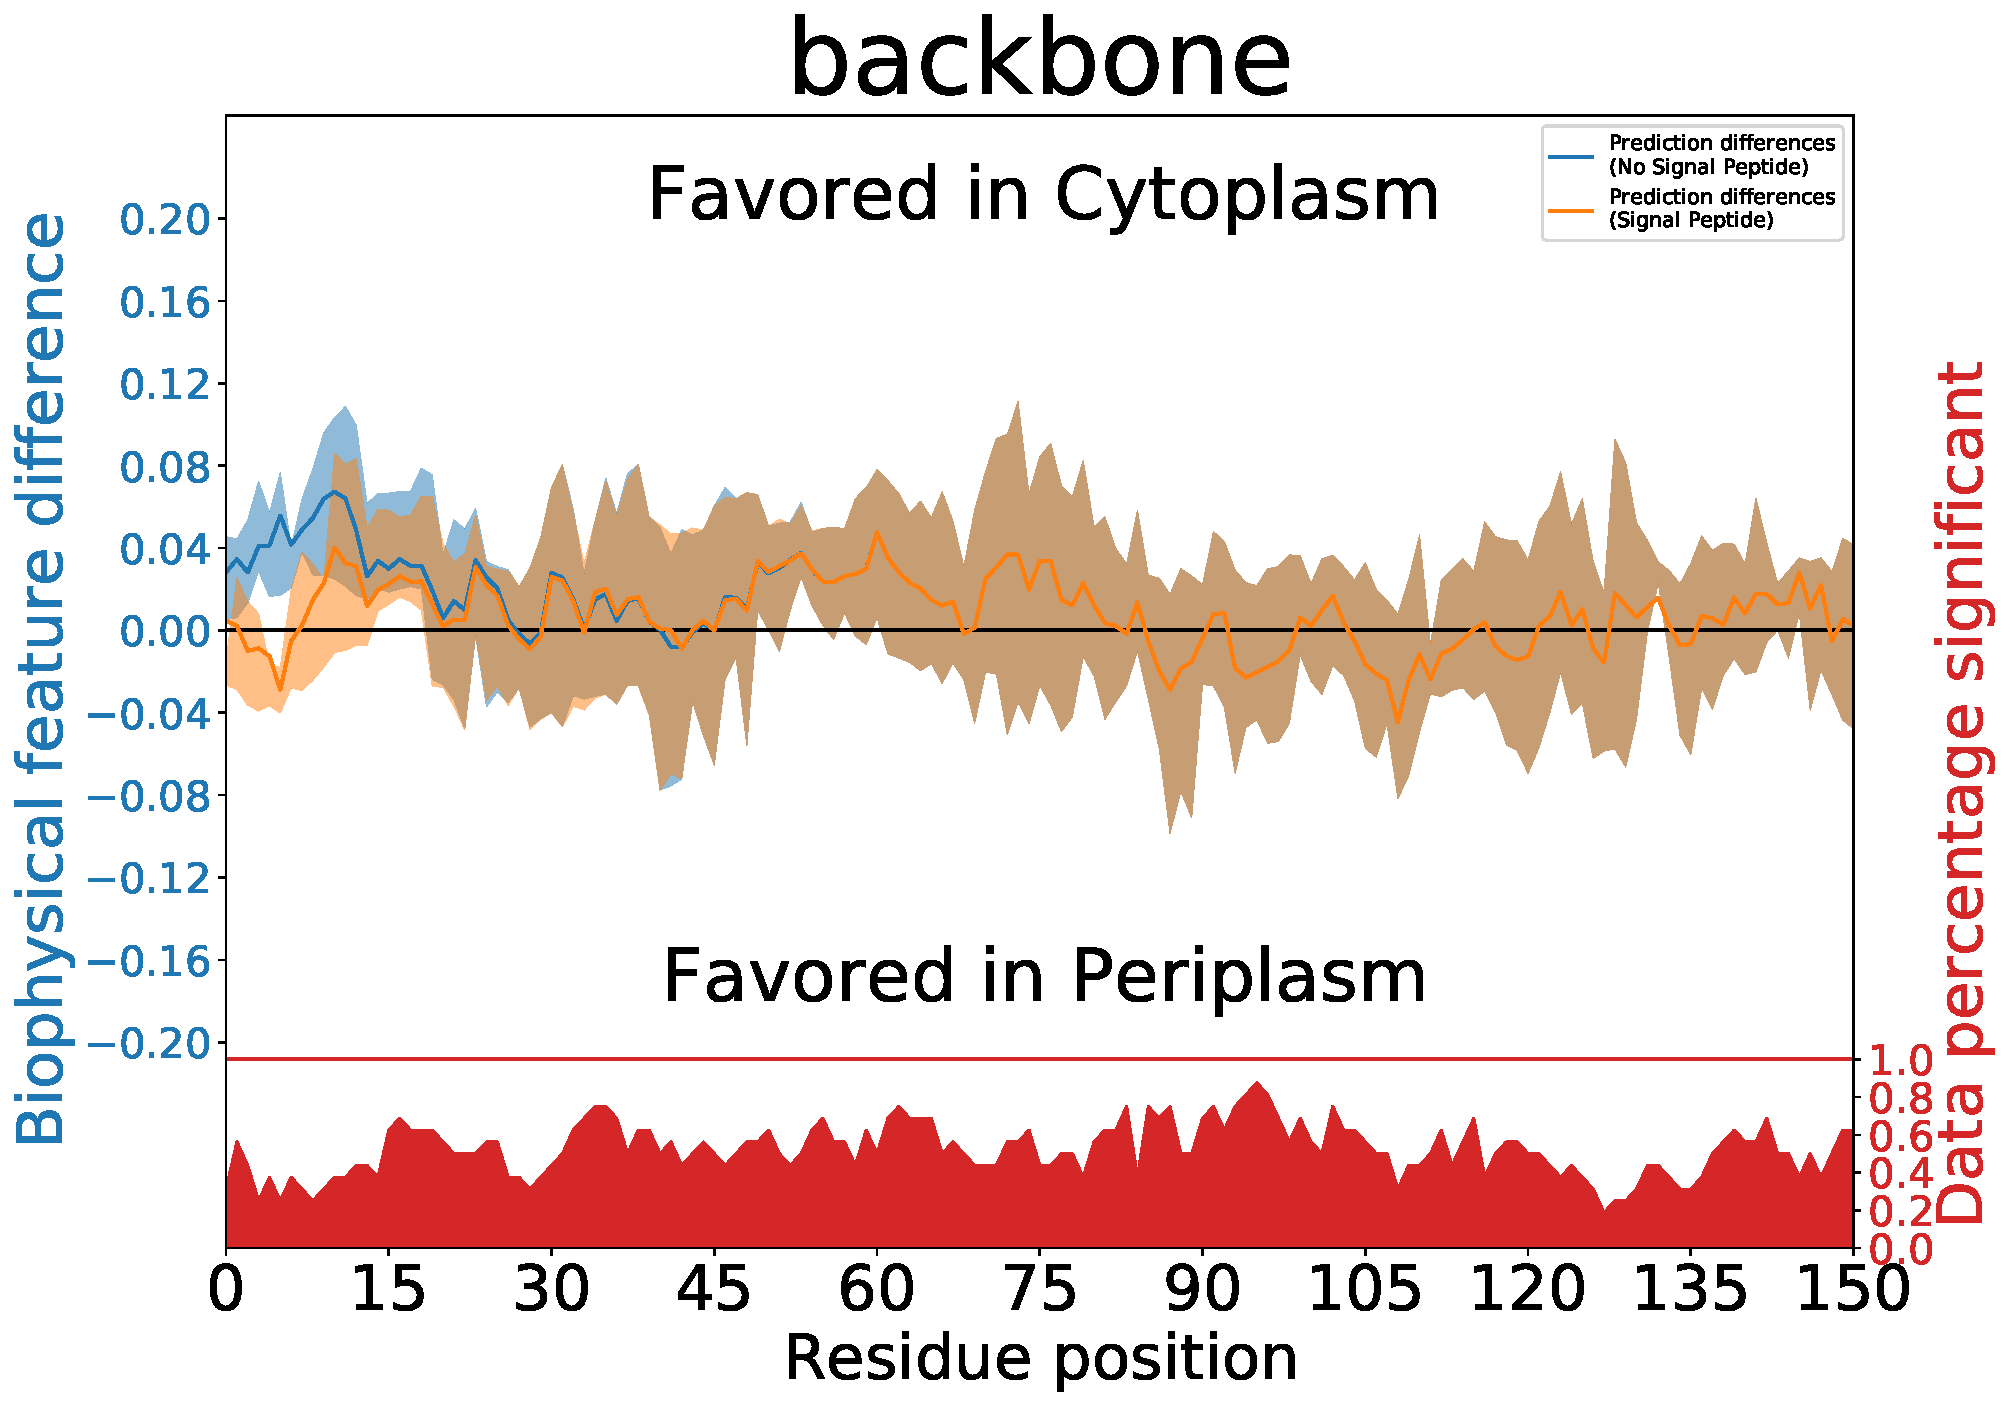
\includegraphics[width=\linewidth, height=0.34\textheight, keepaspectratio]
	{./results/twins/img/backbone.pdf}
		\caption{}
		\label{fig:twin_backbone}
	~\end{subfigure}
	\newline
	~\begin{subfigure}[b]{\linewidth}
			\centering
			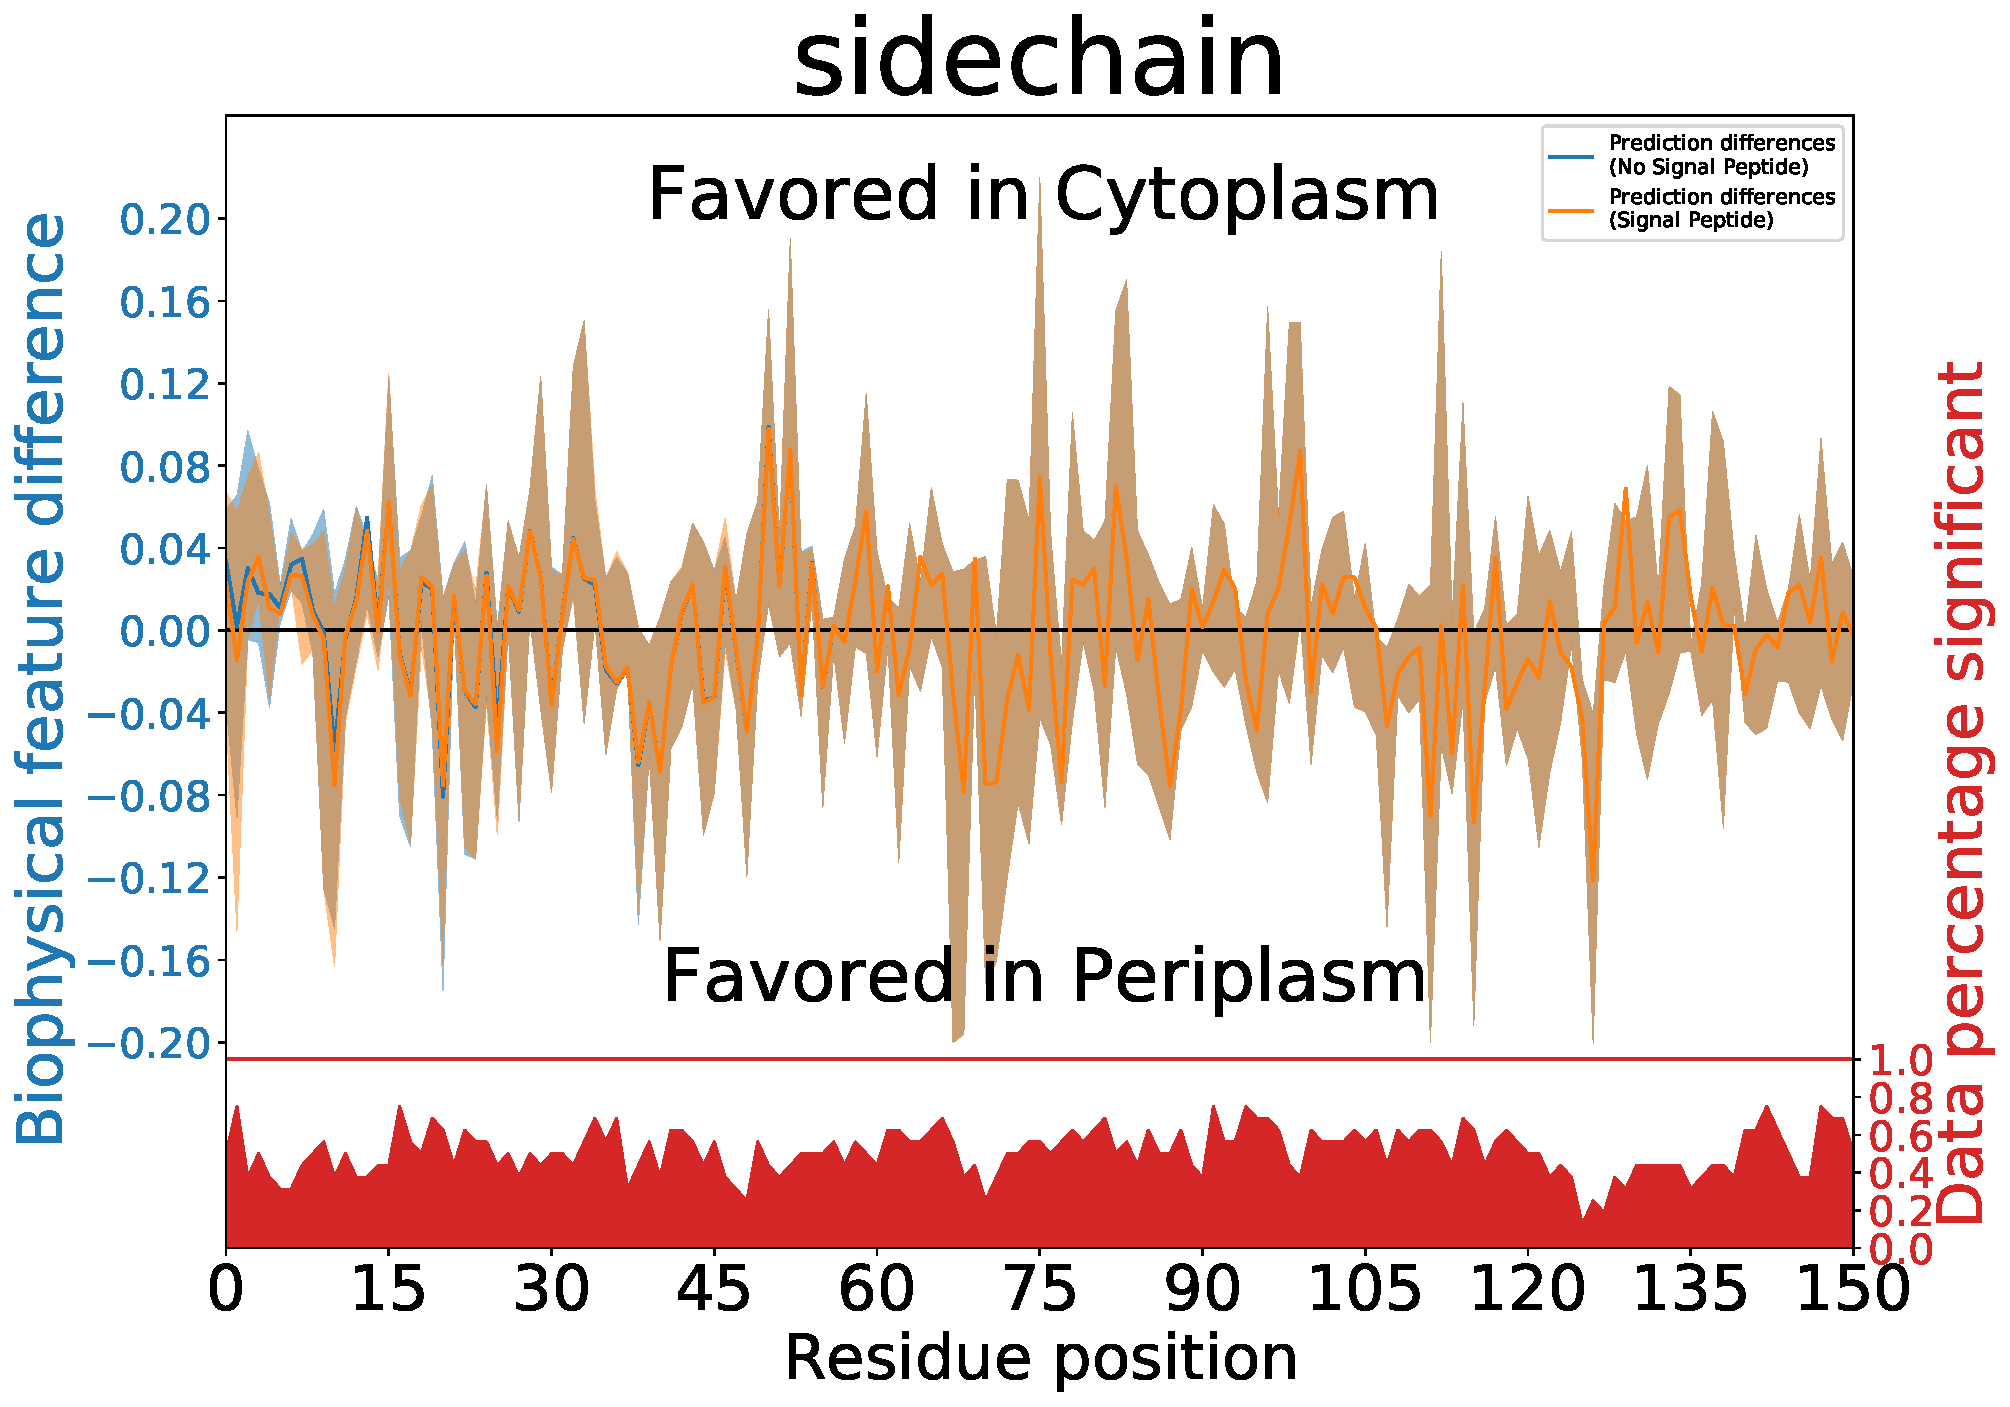
\includegraphics[width=\linewidth, height=0.34\textheight, keepaspectratio]
	{./results/twins/img/sidechain.pdf}
		\caption{}
		\label{fig:twin_sidechain}
	~\end{subfigure}
	\caption{
	\textbf{Difference in biophysical features between twins (first 150 residues)}
The difference of biophysical feature values is plotted in function of residue position.
The full line shows the median, the edge of the coloured area the quartiles,
75 percent of the observations fall within the coloured area.
Only significant differences were included (Wilcoxon-ranksum, P-value < 0.05).
To indicate how many observations of the 16 twins were included,
the red area at the bottom of the graphs gives a ratio between 0 and 1 for each position.
The Y-axis should be interpreted in the following way:
positive differences mean that cytoplasmic proteins tend to have a higher value for a certain property,
negative differences when the periplasmic proteins have a higher value.
Distinction is made between predictions with signal peptide (orange) and without signal peptide (blue).
Signal peptides themselves are not included in the graph.
}
~\end{figure}
